\documentclass[12pt,a4paper,oneside]{book}

\usepackage{algorithm}
\usepackage{algpseudocode}
%\usepackage{algorithmic}
\usepackage{amsmath}
\usepackage{graphics}
\usepackage{epsfig}
% border setting
\usepackage[ top=2.5cm,bottom=2.5cm,left=2.5cm,right=2.5cm ]{ geometry }

% The default for LaTeX is to have no indent after sectional headings, like \chapter and \section. ()
\usepackage{indentfirst}

% http://tex.stackexchange.com/questions/28333/continuous-v-per-chapter-section-numbering-of-figures-tables-and-other-docume
\usepackage{chngcntr}
\counterwithout{figure}{chapter}
\counterwithout{table}{chapter}

% This prevents placing floats before a section
\usepackage[section]{placeins}
\let\Oldsubsection\subsection
\renewcommand{\subsection}{\FloatBarrier\Oldsubsection}

% source code hightlighting
\usepackage{listings}
\lstset{
  numbers=left,
  stepnumber=1,
  firstnumber=1,
  captionpos=b,
  tabsize=2,
  basicstyle=\small,
  numberfirstline=true
}

% setting the page number to footer
\usepackage{fancyhdr}
\fancyhf{}
\cfoot{\thepage}
\pagestyle{fancy}
% no header and footer bar
\renewcommand{\headrulewidth}{0pt}
\renewcommand{\footrulewidth}{0pt}

% setup bibliography
\usepackage[sorting=none,backend=bibtex]{biblatex}
\addbibresource{reference.bib}

% line height setting
\linespread{1.5}
\usepackage{setspace}

% Graphics settings
\usepackage{graphicx}
\graphicspath{ {./figures/} }

\usepackage{background}
\newcommand\DeactivateBG{\backgroundsetup{contents={}}}
\newcommand\ActivateBG{
  \backgroundsetup{
      contents={
\includegraphics[]{logo.jpg}},
      scale=1,
      opacity=0.4,
      angle=0
  }
}

\usepackage{comment}

% do not place figure at the middle of a empty page
\makeatletter
\setlength{\@fptop}{0pt}
\makeatother

% Chinese typesetting
\usepackage{xeCJK}
%\setCJKmainfont{SourceHanSansTW-Light.otf}
\setCJKmainfont[
  BoldFont={SourceHanSansTW-Normal.otf},
  ItalicFont={SourceHanSansTW-Light.otf}
]{SourceHanSansTW-Light.otf}
\newcommand{\myHuge}[1]{\fontsize{40}{50} #1}

\newcommand{\chineseTitle}{中文題目}
\newcommand{\englishTitle}{英文題目}

\newcommand{\studentCnName}{葉家郡}
\newcommand{\studentEnName}{Jia-Jun Yeh}
\newcommand{\advisorCnName}{黃世昆}
\newcommand{\advisorEnName}{Shih-Kun Huang}

\usepackage{pdfpages}
\DeclareMathOperator*{\argmax}{arg\,max}
\begin{document}

\pagenumbering{gobble} % disabling page numbering

\ActivateBG

\begin{titlepage}
  \begin{center}
    \myHuge \textbf{國立交通大學}    \\[0.25cm]

    \Huge \textbf{資訊科學與工程研究所} \\[0.25cm]

    \Huge \textbf{碩士論文} \\[1cm]
	
    \LARGE \chineseTitle{} \\[0.5cm]

    \LARGE \englishTitle{} \\
  \end{center}

  \vspace{\fill}

  \begin{tabular}{c l}
    {\makebox[8em][s]{\LARGE 研究生}}   & \LARGE :\studentCnName{}    \\[0.5cm]
    {\makebox[8em][s]{\LARGE 指導教授}} & \LARGE :\advisorCnName{} \hspace{0.1cm} 教授\\
  \end{tabular}

  \vspace{3cm}

  \begin{center}
    {\LARGE 中華民國  105 年 7 月}
  \end{center}
\end{titlepage}

\begin{titlepage}
  \begin{center}
    \LARGE \chineseTitle{}  \\
    \LARGE \englishTitle{}  \\[1.5cm]
  
    \Large
    \begin{tabular}{c l c c l}
    研究生   & :\studentCnName{} & \hspace{3cm}  & Student  & :\studentEnName{} \\
    指導教授 & :\advisorCnName{} & \hspace{3cm}  & Advisor  & :\advisorEnName{}\\
    \end{tabular}
    \\[1.5cm]
    國立交通大學 \\
    資訊科學與工程研究所 \\
    碩士論文 \\[1cm]
	
    \begin{singlespace}
    A Thesis Submitted to Institute of Computer Science and Engineering College of Computer Science National Chiao Tung University in Partial Fulfillment of the Requirements for the Degree of Master in Computer and Information Science \\
    July 2016 \\
    \studentEnName{}, Taiwan \\
    \end{singlespace}

  \end{center}

  \vspace{\fill}

  \begin{center}
    {\LARGE 中華民國  105 年 7 月}
  \end{center}
\end{titlepage}

\DeactivateBG

% 放審定書和授權書
% \includepdf[pages={1-2}]{auth.pdf}

\ActivateBG

\begin{titlepage}
  \begin{center}
  	\LARGE 
    \begin{singlespace}    
      \textbf{\chineseTitle{}} \\[0.5cm]
    \end{singlespace}
    
    \begin{singlespace}    
    \begin{tabular}{r l}
    	學生     & :\studentCnName{}  \\
        指導教授  & :\advisorCnName{} \hspace{0.1cm} 教授 \\[0.5cm]
    \end{tabular}
    \end{singlespace}

    國立交通大學資訊科學與工程研究所碩士班 \\[0.5cm]
    \makebox[4em][s]{摘要} \\[0.5cm]
    	
  \end{center}
  \normalsize 
  \hspace{0.6cm} 在程式自動化測試與分析上,符號執行(symbolic execution)是目前經常被使用的一種方法,由於符號執行會紀錄並模擬出程式執行時的所有可能路徑,其數量會以指數的數量級成長,最終耗盡所有運算資源,這個問題被稱為路徑爆炸問題(path explosion problem);因此我們需要在有限的資源內採取某些策略來優先計算較有價值的路徑,在本篇論文中我們提出使用以蒙地卡羅搜尋樹為基礎的搜尋策略來解決這個問題,並比較它與其他傳統策略如深度優先搜尋(DFS)、廣度優先搜尋(BFS)的效率。
  \\[0.7cm]
  關鍵字:Monte Carlo Tree Search(MCTS), Upper Confidence Bounds for Trees (UCT), symbolic execution
\end{titlepage}
\begin{titlepage}
  \begin{center}
    \LARGE
    \begin{singlespace}
  	 \textbf{\englishTitle{}} \\[0.5cm]
    \end{singlespace}
    
    \begin{singlespace}
    \begin{tabular}{r l}
    	Student     & : \studentEnName{}  \\
        Advisor  & : Dr. \advisorEnName{} \\[0.5cm]
    \end{tabular}
    \end{singlespace}
	
    \begin{singlespace}
    Institute of Computer Science and Engineering National Chiao Tung University\\[0.5cm]
    \end{singlespace}
    \textbf{ABSTRACT} \\[0.5cm]
    	
  \end{center}
  \normalsize 
  \hspace{0.6cm} Symbolic execution is a technology that is often used today in program automation testing and analysis. Since symbol execution traces and simulates all possible paths when a program executes, its number grows exponentially. This problem is called the path explosion problem. Therefore, we need to take some strategies within the limited resources to give priority to the more valuable path. In this paper, we propose to use The Carlo search tree-based search strategy solves this problem and compares it with other classic strategies such as depth-first search (DFS) and breadth-first search (BFS).
  \\[0.7cm]
  Keywords:Monte Carlo Tree Search(MCTS), Upper Confidence Bounds for Trees (UCT), symbolic execution
\end{titlepage}

\tableofcontents
\listoffigures
\listoftables

% 9/30
\chapter{Introduction} \pagenumbering{arabic} % enabling page numbering

在現今的軟體開發中,程式碼數量動輒數萬行,系統的複雜度也越來越高,傳統驗證程式正確性的方式如unit testing、code review等等...受限於人工而相當有限;在硬體計算能力突飛猛進的現代,自動化測試的方式又逐漸成為顯學,如fuzzing、symbolic execution...能夠自動尋找程式中可能的漏洞,其中symbolic execution是一種模擬執行的方法,它將程式的使用者輸入視為符號,並把程式執行過程和分支條件轉換為限制式,藉由求解限制式來獲得欲執行該路徑所需的使用者輸入為何;由於symbolic execution在遇到分支時會複製出一條新的路徑,兩條路徑分別探索執行if時和執行else時的狀態,因此路徑數量會以指數的數量級成長,造成探索路徑需要花費巨大的運算資源,這個問題被稱為path explosion problem,這篇論文欲以蒙地卡羅樹搜尋演算法來找出探索價值較高的路徑,使得symbolic execution能使用較短的時間內獲得更高的程式執行覆蓋率。

蒙地卡羅樹搜尋(Monte Carlo tree search)被廣泛的運用在遊戲人工智慧中,例如西洋棋、黑白棋、圍棋等等的棋盤遊戲,在2016年AlphaGo(一個結合蒙地卡羅樹搜尋和深度學習的圍棋AI程式)擊敗世界棋王後,更是一度引起相當多的討論;此演算法主要的精神在於對一棵樹,選擇子結點並嘗試用模擬的方式估計該結點的價值。和symbolic execution相當類似的地方在於同為需要探索一棵樹,而且要避免探索一些我們不感興趣或是沒有必要探索的路徑,例如無窮迴圈的狀況;我們認為結合蒙地卡羅樹搜尋做為symbolic execution挑選路徑執行的演算法,相較於傳統的深度優先搜尋法或廣度優先搜尋法,能有較佳的搜尋效率。

% \cite{thesis}.

% 9/30
\chapter{Background}

在這個章節將簡要介紹Symbolic execution與其遇到的問題,還有蒙地卡羅樹搜尋演算法的流程和優點。

\section{Symbolic execution}

% 說明symbolic execution的流程和精神
在本篇論文中所提及的Symbolic execution為Dynamic symbolic execution(又名為Concolic execution),首先由K. Sen\cite{sen2007concolic}提出,和基於其想法實作的程式DART\cite{godefroid2005dart}、CUTE\cite{sen2005cute},而其近年又分為兩種類型,需要程式原始碼的code-based symbolic execution,如KLEE\cite{cadar2008klee}和不須程式碼而直接分析程式執行檔的binary-based symbolic execution如S2E\cite{chipounov2012s2e}、Mayhem\cite{cha2012mayhem};symbolic execution engines在分析程式時會將其載入並先轉換為intermediate representation (IR),接著會將使用者輸入(例如標準輸入、檔案、命令列參數)標記為symbolic變數,接著模擬程式的執行過程,將執行過程中遇到的程式碼轉換為數學邏輯限制式的形式,當在模擬的過程中遇到分支條件時,便複製出一條新的路徑,分別追蹤該分支條件為真和為假時的情況;當模擬執行結束時,把先前蒐集的邏輯限制式利用solver求解(如:SMT\cite{vanegue2012smt}、Z3\cite{Z3}等等),以取得欲執行該路徑所需的實際輸入值;透過這個流程理論上我們可以追蹤所有的執行路徑,探索是否有不當的輸入值能觸發程式崩潰。

\section{Path Exploration}

% 說明symbolic execution中的路徑探索問題
雖然Symbolic execution理論上能夠探索所有執行路徑,但在探索的過程中可能會遭遇到一些問題:當分支條件取決於symbolic變數時,很有可能兩邊的條件都有可能成立,這意謂著程式必須複製並分別維護兩條路徑,直到發現該路徑無解為止,當路徑被不斷的複製就產生了路徑爆炸問題(path explosion problem)。

\section{Monte Carlo tree search}

MCTS是一種啟發式搜尋演算法,近年來最廣為人知的應用是遊戲AI方面的演算法;Monte Carlo模擬是利用模擬和統計,得到一個近似解,在足夠大量的模擬下,理論上我們可以得到一個跟最佳解非常接近的答案。MCTS套用了這種模擬的方式,維護一棵樹(在遊戲AI中通常是一個遊戲盤面的狀態樹)並統計每個盤面的勝率,期望能只探索部分的樹,而非全部探索完的情況下,就能知道該盤面的勝率。

在\cite{browne2012surveyMCTS}中說明了MCTS演算法的基本流程,如Figure \ref{figMCTS}:

\begin{figure}[h]
\center
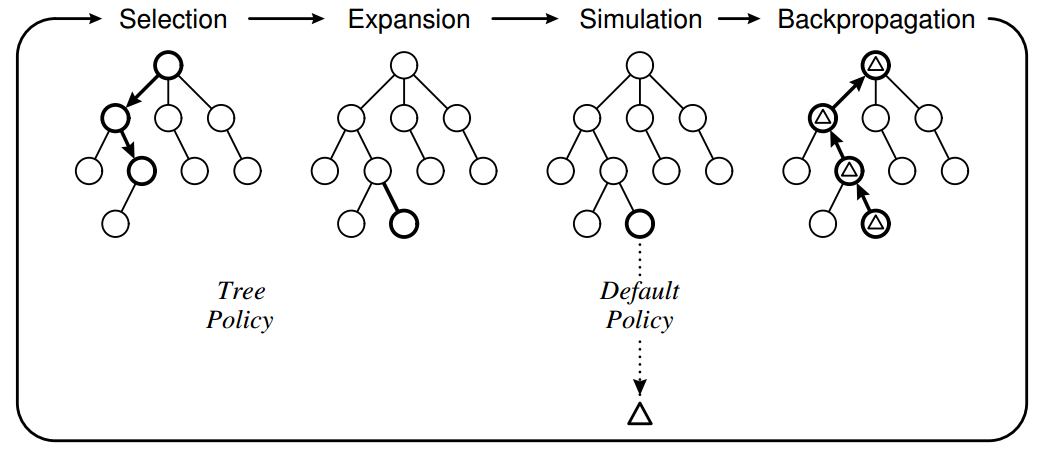
\includegraphics[width=\textwidth,height=\textheight,keepaspectratio]{figures/mcts2.PNG}
\caption{Monte Carlo Tree Search \label{figMCTS}}
\end{figure}

\begin{itemize}
\item \textbf{Selection} 根據設定的\textit{Tree Policy},從根節點開始遞迴性的決定一個目前最需要展開的節點,如Figure \ref{figMCTS}中的Selection部分,以粗框標記出的節點。可展開的節點在這裡定義為狀態尚未終止且有尚未訪問的子節點。
\item \textbf{Expansion} 在選擇的節點上,執行一個合法的動作來新增子節點,如Figure \ref{figMCTS}中的Expansion部分,在挑選的節點下新增一個節點。
\item \textbf{Simulation} 從這個新增的節點上使用\textit{Default Policy}來進行模擬執行,產生結果。
\item \textbf{Backpropagation} 模擬的結果會回饋到步驟1所選擇路過的那些節點上,更新他們的統計數據。
\end{itemize}

在這邊有兩個policy:\textit{Tree Policy}代表的是如何決定要選擇和新增節點的演算法。\textit{Default Policy}則是從該節點的狀態模擬對局直到獲得勝負結果。雖然這兩個Policy也可以簡單的使用隨機方式決定,但適當的演算法有助於強化MCTS的準確度,如\cite{Intro2MCTS}便指出,Tree Policy可以使用upper confidence bound (UCB)演算法來取代隨機挑選,當可能的選擇有很多,卻只有少數一兩個有可能被選擇時,隨機選擇不太容易挑到,而造成模擬的結果不精準,如果我們把盤面的位置當成吃角子老虎機,視為multi-armed bandit problem來處理的話,會比原本的隨機選擇好;另外他也指出模擬時除了用這些簡單的方法,也可以使用更耗費資源的啟發式邏輯和評價方式,在對於higher branching factor的遊戲會有較好的效果。

\chapter{Design}

傳統的MCTS演算法是為了要在特定時間或電腦資源使用量內做出某個決策,利用隨機模擬與統計的方式尋找出一個最佳解,如何最有效的擴展空間狀態樹是我們的演算法可以仿效之處。對symbolic execution而言,目標就變成如何達到更高的執行覆蓋率,以盡量的挖掘出可能的漏洞。Algorithm 1 為我們設計的演算法主體,其中有兩項可自行定義的參數$N$和$\alpha$,$N$代表的是在\textit{Default Policy}中模擬執行的次數,越多次模擬的結果會更精準,但也需要花費更多的時間;而$\alpha \beta$是為了調整模擬生成之children的value $Q$,$\frac{|V-B|}{N}$為children $p_c$可能增加執行覆蓋率的期望值,$|p_c|$為$p_c$執行過的basic blocks數量。

\begin{algorithm}[h]
  \caption{applying UCT algorithm to symbolic execution}
  \begin{algorithmic}[1]
  	\Function{Search}{$p_r$}
    \State set $p_r$ as root of Tree $T$
    \State $B \leftarrow \emptyset$
    \While {within computational budget}
      \State $p$ $\leftarrow$ TreePolicy($T$)
      \State $B \leftarrow B \bigcup p$
      \State $S$ $\leftarrow$ step($p$)
      \For{each path $p_c \in S$}
      	\State $V \leftarrow$ DefaultPolicy($p_c$)
        \State $Q(p_c) \leftarrow \alpha \frac{|V-B|}{N} + \beta|p_c|$
        \State add a new child $p_c$ to $p$
      \EndFor
      \State BackPropagation($p$)
    \EndWhile
    \EndFunction
  \end{algorithmic}
\end{algorithm}

\begin{algorithm}[h]
  \caption{Policies for our algorithm}
  \begin{algorithmic}[]
    \Function{TreePolicy}{$T$}
    	\State $n \leftarrow$ root of $T$
        \While {$n$ is not terminated}
        	\If{$n$ is expandable}
            	\State \Return {$n$}
            \Else
            	\State $n \leftarrow BestChild(n,C)$
            \EndIf
        \EndWhile
    \EndFunction
    \item[]
	\Function{DefaultPolicy}{$p$}
    	\State $V \leftarrow \emptyset$
        \For{$i=1$; $i<N$; $i++$}
          \State $v \leftarrow$ find vertex at CFG($p$'s addr)
          \For{$j=1$; ($j<M$)and($v$ has any edge); $j++$}
              \State add $v$ to $V$
              \State $v \leftarrow$ random pick a vertex which $v$ directed to
          \EndFor
        \EndFor
        \State \Return $V$
    \EndFunction
    \item[]
    \Function{BestChild}{$p,C$}
    	\State $Q_{max} \leftarrow \operatorname*{arg\,max}_{p_c \in p} Q(p_c)$
    	\State \[ \Return \argmax_{p_c \in p} \frac{Q(p_c)}{Q_{max}}+C\sqrt[]{\frac{2\ln N(p)}{N(p_c)}} \]
    \EndFunction
    \item[]
    \Function{BackPropagation}{$v$}
    \While{$v$ is not null}
    	\State N($v$) += 1
		\State Q($v$) $\leftarrow$ average of Q($v$'s children)
    \State $v \leftarrow$ parent of $v$
    \EndWhile
    \EndFunction
  \end{algorithmic}
\end{algorithm}
  
Algorithm 1 在執行時除了紀錄MCTS樹的資料,也會記錄目前已經執行過的block來計算覆蓋率和判斷期望值,首先經由\textit{TreePolicy}選出應該被展開的節點$p$,接著把該節點執行過的blocks加進集合$B$中,接著用symbolic execution的step往前執行一個block,他會回傳增加這個block後的結果,根據該block的分枝跳轉方式,可能為1到多條path。我們要將所有產生的path都進行模擬以計算出$p$的value $Q$,首先將產生出的path $p_c$利用\textit{DefaultPolicy}模擬出未來可能的執行路徑,並以公式計算出$Q$,並將$p_c$新增到$T$中視為$p$的children;最後於\textit{BackPropagation}時,以children的value平均作為$p$的value,並將此結果一路更新到root節點。
  
在演算法中有幾項參數來影響選擇的策略,針對不同的程式特性來設定有可能得到更好的性能。計算$Q$時的$\alpha$主要控制的是增加覆蓋率的期望值,由於路徑的模擬是根據CFG來猜測,如果產生的CFG不正確或程式的實際執行狀況和模擬的結果有落差,期望值就會變得不準確,相對的對於簡單的小程式,模擬的準確度有可能是較高的,因此適當的調整$\alpha$可以修正模擬的數據;而$\beta$是為了因應遇到大量迴圈或strcmp這類function的措施,由於進入迴圈容易產生大量的分枝,會讓path數量一下子成長很多,\textit{TreePolicy}在選擇時也容易被混淆,我們透過計算該path已經執行過的basic blocks數量,讓演算法在挑選時偏好已經執行比較多數量的path,因為較多的數量也意味著較有可能離開迴圈。

\textit{TreePolicy}中還有一個參數$C$,其影響的是expolitation和exploration,也就是程式該往較深的點進行計算,還是選擇較少被計算過的點,不過這個數值在branching factor高時較有效,而我們產生出的path常常只有1至2個,所以這個參數的影響並不大,唯一會影響的是當某個節點尚未被計算過任何一次的時候,$N(p_c)$為0,根號內的數值會是無限大,程式就一定會選擇該節點來進行計算。
  
最後是\textit{DefaultPolicy}的參數$N,M$,$N$是要進行幾次模擬,而$M$是避免程式進入無窮迴圈,當到達一定數字時會強制中斷模擬,對於較小的程式可以選擇較小的數字,而較複雜的程式可以選擇比較大的數字來增加其準確性,但也相對的花費更多時間。

\chapter{Evaluation}

% 9/30
\chapter{Related Work}

\section{Path Selection Problem}

在\cite{sharma2012critical}\cite{schwartz2010all}中對symbolic execution所做的概述,提及了幾項目前的挑戰,其中最大的問題就是路徑選擇問題(path selection problem),當路徑爆炸問題已成一個不可避免的問題,目前已經提出的幾種解決方式如:KLEE\cite{cadar2008klee}中提出的深度優先搜尋法來優先探索最深的路徑,中便使用這種作法,但很有可能被困在無限迴圈而進行了無效的探索。\cite{sen2007concolic}提出的concolic testing,除了以symbolic execution執行,也會使用具體的輸入真正執行程式來蒐集執行路徑,\cite{sen2005cute}就使用了這種作法。而KLEE\cite{cadar2008klee}也支援隨機挑選路徑的方式來避免進行了無效的探索。

另外如driller\cite{stephens2016driller}結合了AFL\cite{AFL}的fuzzing技術,它將使用者輸入分類為需要特定值的特定輸入(specific input)和可接受各種數值的通用輸入(general input),並透過symbolic execution engine和fuzzing engine的切換來解決各自不擅長的部分。而s2e\cite{chipounov2012s2e}則是利用選擇性的symbolic execution,避免連同其他函式庫也一起分析,造成路徑數量大量增長。另外也有針對路徑成長,檢查其可滿足性(satisfiability)並做動態剪枝的方法\cite{PathPruning}。

\section{MCTS and Game AI}

Monte Carlo方法是一種隨機取樣的方法,在1987年由Bruce Abramson提出\cite{mcmethod}。而在1989年,Monte Carlo tree search由W. Ertel, J. Schumann和C. Suttner提出,用來改善搜尋演算法的時間如DFS、BFS等等。而在1993年B. Brügmann首先將Monte Carlo方法用於圍棋上\cite{mc_go},直到2006年這個方法才由Rémi Coulom真正被命名為Monte Carlo tree search\cite{MCTS_naming}。之後 L. Kocsis and Cs. Szepesvári以MCTS為基礎發表了upper confidence bound 1 applied to trees (UCT)演算法\cite {UCT}。在2015年由Google Deepmind研發的圍棋AI AlphaGo\cite{alphago},使用MCTS和deep learning演算法,擊敗了人類職業選手,頓時之間AI和機器學習又成為電腦科學界的顯學。

\chapter{Conclusion}

\newpage

\printbibliography[title={References}]

\end{document}
